\section{Analysis of vegetation density}
\label{sec:vegetation_analysis}

\subsection{Spectral Vegetation Indices}
\WIP{
\cite{glv03}
Spectral vegetation indices (SVI) are indicator for vegetation density. based on fact, that healthy vegetation absorbs most of visible red and blue light, but reflect green and NIR light. in fact, reflections of green lights are significantly higher than other spectrums. other materials dont show this bump in green spectrum, instead show steady rise in reflectance as wavelengths increase.

SVIs compare difference between visible and NIR light. the greater the difference, the greater the amount of green vegetation in the scene. There are various indices that each combine data from multiple spectral bands to a single value indicating the vegetation health and density. Most of them use simple algebraic formulas. Some of the commonly used indices are now introduced.
}

\subsubsection{Ratio Vegetation Index}
\WIP{
\cite{glv03}
Ratio Vegetation Index (RVI) is simply ratio between NIR light and red light (equation \ref{eq:rvi}). Values for non-vegetation area are generally around $1$, because similar reflectance of NIR and red light. index can not go below $0$ for practical reasons (can not be less than no reflectance). Higher means more vegetation, high values typically reaching up to magnitude of $30$. however, there is no upper bound.

\begin{equation}
    \text{RVI} = \frac{\text{NIR}}{\text{Red}}
    \label{eq:rvi}
\end{equation}
}

\subsubsection{Normalized Difference Vegetation Index}
\WIP{
\cite{gisg_ndvi20}
NDVI ranges from $-1$ to $1$. Negative values indicate high probability for water. Positive values imply vegetation, where higher values mean more/denser vegetation. Values around 0 just tell that there is no vegetation, but does not tell about land cover. Could be desert, rocks or urban areas.


\cite{measuring_vegetation00}
first use of vegetation analysis was driven by National Oceanic and Atmospheric Administration (NOAA), US agency focusing on conditions of the environment. They launched satellites carrying an Advanced Very-High-Resolution Radiometer (AVHRR) instrument to measure earth's reflectance in five spectral bands. Two of sensors are sensitive to wavelengths ranging from $550$ to $700$ nanometers (red light), an $730$ to $1000$ nanometers (near-infrared light). the NDVI is based on those two values. \ref{eq:ndvi} shows formula to calculate NDVI.

\begin{equation}
    \text{NDVI} = \frac{\text{NIR}-\text{Red}}{\text{NIR}+\text{Red}}
    \label{eq:ndvi}
\end{equation}
}

\subsubsection{Enhanced Vegetation Index}
\WIP{
better measuring instruments were launched, for example Terra\footnote{see \url{https://terra.nasa.gov/}} mission of National Aeronautics and Space Administration (NASA). satellite carries a sensor called Moderate Resolution Imaging Spectroradiometer (MODIS). instruments capture wavelengths from $400~\text{nm}$ to $14400~\text{nm}$ in resolution up to $250$ meters \cite{modis2002}. more accurate data led to adjustments in calculations, eventually resulting in Enhanced Vegetation Index (EVI).

Enhanced Vegetation Index similar to NDVI. Has some additional factors to correct atmospheric conditions and background noise. This means, EVI is more sensitive in areas with dense vegetation.

Equation \ref{eq:evi} shows how EVI is calculated. $C_1$ and $C_2$ are coefficients to reduce aerosol influences in red color band using the blue color band. $L$ is adjustment to address canopy background noise. $G$ value is gain factor for linear scale. Values chosen in original mission are $C_1=6$, $C_2=7.5$, $L=1$ and $G=2.5$. \cite{modis2002}

\begin{equation}
    \text{EVI} = G * \frac{
    \text{NIR}-\text{Red}
    }{
    \text{NIR} + C_1 * \text{Red} - C_2 * \text{Blue} + L
    }
    \label{eq:evi}
\end{equation}
}

\subsubsection{Soil-Adjusted Vegetation Indices}
\WIP{
another approach to improve NDVI is \emph{Soil Adjusted Vegetation Index} (SAVI) \cite{savi88}. Huete found NDVI to be unstable with factors like soil color and moisture. Introduced a canopy background adjustment factor $L$ to correct unwanted influence of soil variations. In his experiments, he found value of $L=0.5$ works best to eliminate side effects without further calibration. equation \ref{eq:savi} shows exact calculation.

\begin{equation}
    \displaystyle
    \text{SAVI} =
    \bigg(
    \frac{\text{NIR} - \text{Red}}
    {\text{NIR} + \text{Red} + L}
    \bigg) * \big(1 + L \big)
    \label{eq:savi}
\end{equation}

one issue with SAVI is that proper soil adjustment depends on vegetation density. Without prior knowledge regarding vegetation it is hard to find value of $L$ that works good for everything. Qi et~al. presented a functional $L$ factor to replace in SAVI. Calculation shown in \ref{eq:msavi}. entire derivation is to be found in \cite{msavi94}.

\begin{equation}
    \displaystyle
    \text{MSAVI} = \frac
    {
    2 \text{NIR} + 1
    - \sqrt{
    \big(2 \text{NIR}\big)^2
    - 8 \big(\text{NIR} - \text{Red}\big)
    }
    }
    {2}
    \label{eq:msavi}
\end{equation}
}

\subsection{Experiments}
\WIP{
\begin{itemize}
    \item compute vegetation indices for some images
    \item compare results to the real landscape in the dataset
\end{itemize}
}

\newcommand{\VegetationIndicesImageWidth}{0.18\textwidth}
% INFO: no upper bound for RVI. Calculated biggest values and interpolated from 0-20 to 0-255 for visualization
\begin{figure}
    \centering

    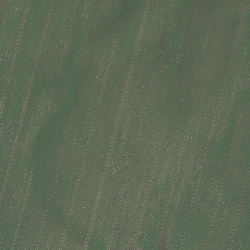
\includegraphics[width=\VegetationIndicesImageWidth]{images/vegetation/original/1} \hfill
    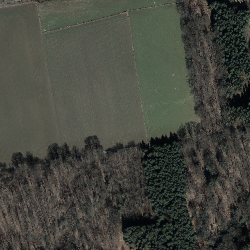
\includegraphics[width=\VegetationIndicesImageWidth]{images/vegetation/original/2} \hfill
    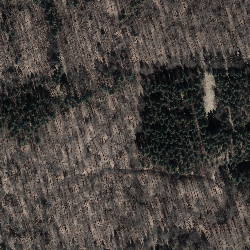
\includegraphics[width=\VegetationIndicesImageWidth]{images/vegetation/original/3} \hfill
    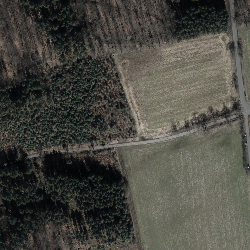
\includegraphics[width=\VegetationIndicesImageWidth]{images/vegetation/original/4} \hfill
    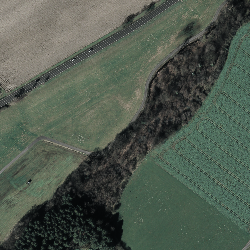
\includegraphics[width=\VegetationIndicesImageWidth]{images/vegetation/original/5}

    \vspace{3mm}
    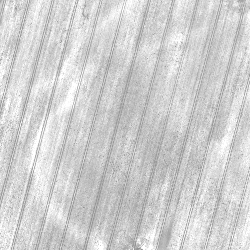
\includegraphics[width=\VegetationIndicesImageWidth]{images/vegetation/rvi/1} \hfill
    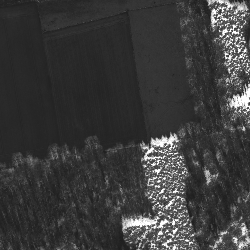
\includegraphics[width=\VegetationIndicesImageWidth]{images/vegetation/rvi/2} \hfill
    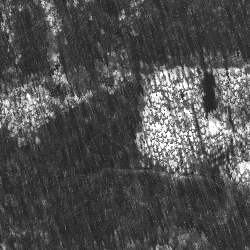
\includegraphics[width=\VegetationIndicesImageWidth]{images/vegetation/rvi/3} \hfill
    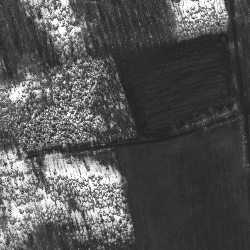
\includegraphics[width=\VegetationIndicesImageWidth]{images/vegetation/rvi/4} \hfill
    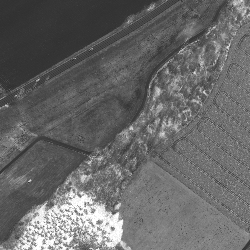
\includegraphics[width=\VegetationIndicesImageWidth]{images/vegetation/rvi/5}

    \caption{Vegetation analysis using RVI}
    \label{fig:vegetation_rvi_examples}
\end{figure}

\begin{figure}
    \centering

    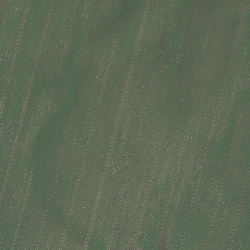
\includegraphics[width=\VegetationIndicesImageWidth]{images/vegetation/original/1} \hfill
    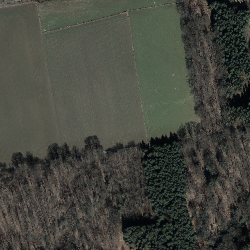
\includegraphics[width=\VegetationIndicesImageWidth]{images/vegetation/original/2} \hfill
    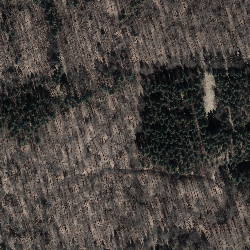
\includegraphics[width=\VegetationIndicesImageWidth]{images/vegetation/original/3} \hfill
    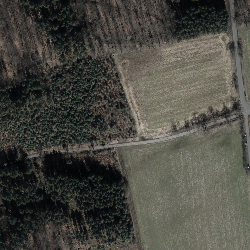
\includegraphics[width=\VegetationIndicesImageWidth]{images/vegetation/original/4} \hfill
    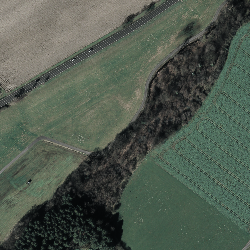
\includegraphics[width=\VegetationIndicesImageWidth]{images/vegetation/original/5}

    \vspace{3mm}
    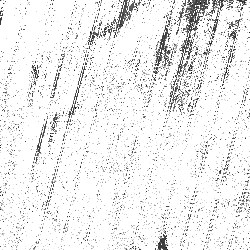
\includegraphics[width=\VegetationIndicesImageWidth]{images/vegetation/ndvi/1} \hfill
    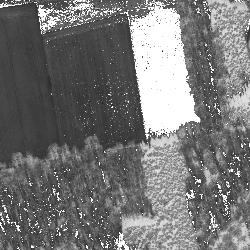
\includegraphics[width=\VegetationIndicesImageWidth]{images/vegetation/ndvi/2} \hfill
    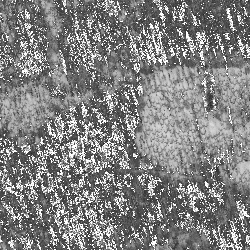
\includegraphics[width=\VegetationIndicesImageWidth]{images/vegetation/ndvi/3} \hfill
    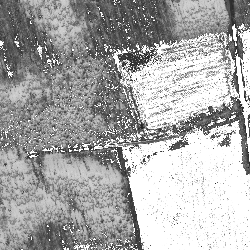
\includegraphics[width=\VegetationIndicesImageWidth]{images/vegetation/ndvi/4} \hfill
    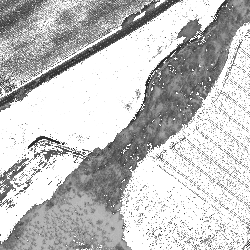
\includegraphics[width=\VegetationIndicesImageWidth]{images/vegetation/ndvi/5}

    \caption{Vegetation analysis using NDVI}
    \label{fig:vegetation_ndvi_examples}
\end{figure}

\begin{figure}
    \centering

    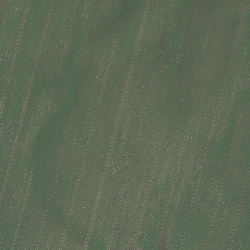
\includegraphics[width=\VegetationIndicesImageWidth]{images/vegetation/original/1} \hfill
    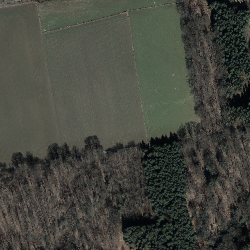
\includegraphics[width=\VegetationIndicesImageWidth]{images/vegetation/original/2} \hfill
    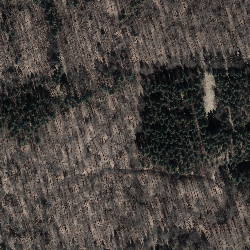
\includegraphics[width=\VegetationIndicesImageWidth]{images/vegetation/original/3} \hfill
    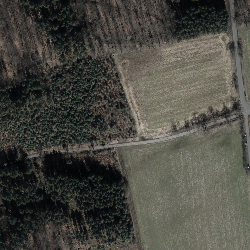
\includegraphics[width=\VegetationIndicesImageWidth]{images/vegetation/original/4} \hfill
    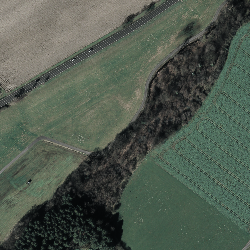
\includegraphics[width=\VegetationIndicesImageWidth]{images/vegetation/original/5}

    \vspace{3mm}
    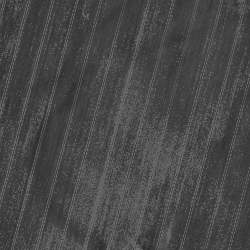
\includegraphics[width=\VegetationIndicesImageWidth]{images/vegetation/evi/1} \hfill
    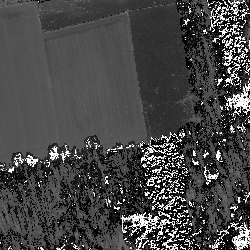
\includegraphics[width=\VegetationIndicesImageWidth]{images/vegetation/evi/2} \hfill
    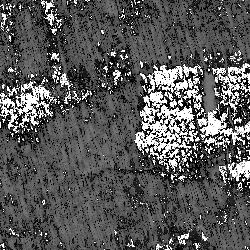
\includegraphics[width=\VegetationIndicesImageWidth]{images/vegetation/evi/3} \hfill
    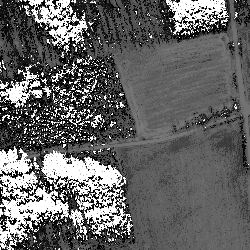
\includegraphics[width=\VegetationIndicesImageWidth]{images/vegetation/evi/4} \hfill
    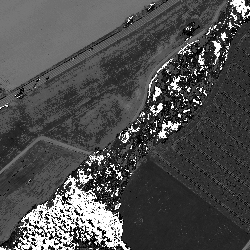
\includegraphics[width=\VegetationIndicesImageWidth]{images/vegetation/evi/5}

    \caption{Vegetation analysis using EVI}
    \label{fig:vegetation_evi_examples}
\end{figure}

% INFO: no bounds for (M)SAVI. Interpolated from SAVI 0-20, MSAVI 0-80
\begin{figure}
    \centering

    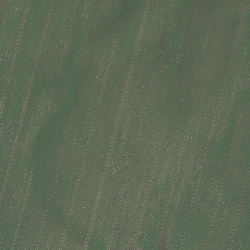
\includegraphics[width=\VegetationIndicesImageWidth]{images/vegetation/original/1} \hfill
    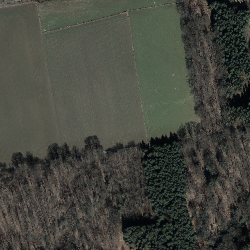
\includegraphics[width=\VegetationIndicesImageWidth]{images/vegetation/original/2} \hfill
    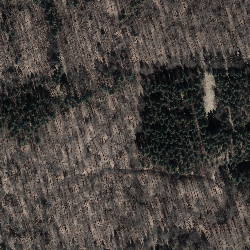
\includegraphics[width=\VegetationIndicesImageWidth]{images/vegetation/original/3} \hfill
    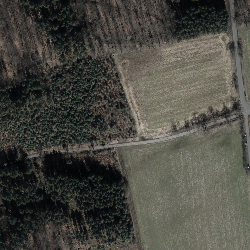
\includegraphics[width=\VegetationIndicesImageWidth]{images/vegetation/original/4} \hfill
    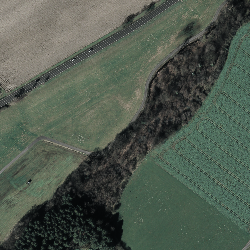
\includegraphics[width=\VegetationIndicesImageWidth]{images/vegetation/original/5}

    \vspace{3mm}
    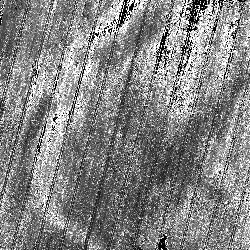
\includegraphics[width=\VegetationIndicesImageWidth]{images/vegetation/savi/1} \hfill
    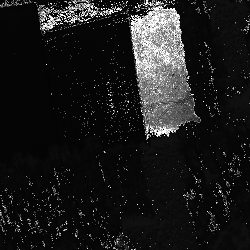
\includegraphics[width=\VegetationIndicesImageWidth]{images/vegetation/savi/2} \hfill
    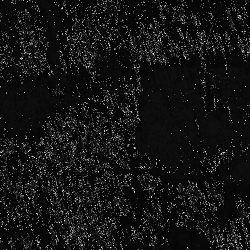
\includegraphics[width=\VegetationIndicesImageWidth]{images/vegetation/savi/3} \hfill
    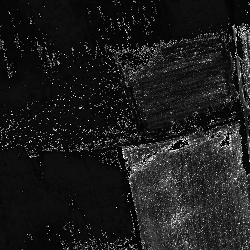
\includegraphics[width=\VegetationIndicesImageWidth]{images/vegetation/savi/4} \hfill
    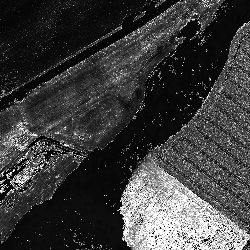
\includegraphics[width=\VegetationIndicesImageWidth]{images/vegetation/savi/5}

    \vspace{3mm}
    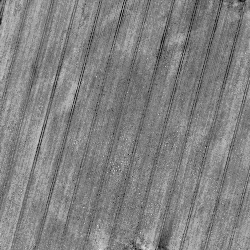
\includegraphics[width=\VegetationIndicesImageWidth]{images/vegetation/msavi/1} \hfill
    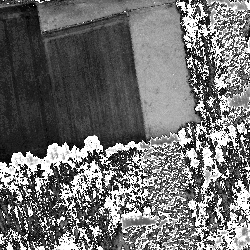
\includegraphics[width=\VegetationIndicesImageWidth]{images/vegetation/msavi/2} \hfill
    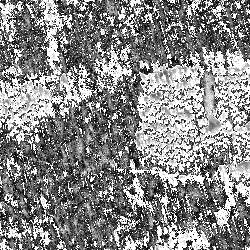
\includegraphics[width=\VegetationIndicesImageWidth]{images/vegetation/msavi/3} \hfill
    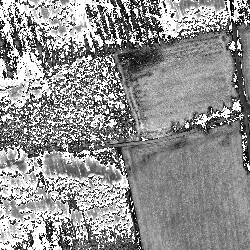
\includegraphics[width=\VegetationIndicesImageWidth]{images/vegetation/msavi/4} \hfill
    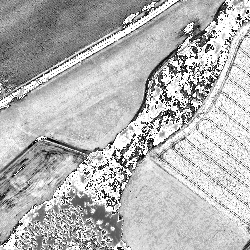
\includegraphics[width=\VegetationIndicesImageWidth]{images/vegetation/msavi/5}

    \caption{Vegetation analysis using SAVI and MSAVI}
    \label{fig:vegetation_savi_examples}
\end{figure}

\subsection{Discussion}
\WIP{
\begin{itemize}
    \item raise concerns about dataset limitation regarding the indices
    \item discuss practical use of those results for identifying emergency landing fields
\end{itemize}
}

\newpage
